\documentclass[sigconf,nonacm,10pt]{acmart}
\usepackage{lmodern}
\usepackage{amssymb,amsmath}
\usepackage{ifxetex,ifluatex}
\usepackage{fixltx2e} % provides \textsubscript
\ifnum 0\ifxetex 1\fi\ifluatex 1\fi=0 % if pdftex
  \usepackage[T1]{fontenc}
  \usepackage[utf8]{inputenc}
\else % if luatex or xelatex
  \ifxetex
    \usepackage{mathspec}
  \else
    \usepackage{fontspec}
  \fi
  \defaultfontfeatures{Ligatures=TeX,Scale=MatchLowercase}
  \newcommand{\euro}{€}
\fi
% use upquote if available, for straight quotes in verbatim environments
\IfFileExists{upquote.sty}{\usepackage{upquote}}{}
% use microtype if available
\IfFileExists{microtype.sty}{%
\usepackage{microtype}
\UseMicrotypeSet[protrusion]{basicmath} % disable protrusion for tt fonts
}{}
\usepackage{hyperref}
\PassOptionsToPackage{usenames,dvipsnames}{color} % color is loaded by hyperref
\hypersetup{unicode=true,
            pdftitle={If a Path is Inflated, and Noone Uses It, Is It Inefficient{[}a{]}?},
            colorlinks=true,
            linkcolor=blue,
            citecolor=blue,
            anchorcolor=blue,
            urlcolor=blue,
            breaklinks=true}
\urlstyle{same}  % don't use monospace font for urls
\usepackage{natbib}
\bibliographystyle{ACM-Reference-Format.bst}
\usepackage{graphicx,grffile}
\makeatletter
\def\maxwidth{\ifdim\Gin@nat@width>\linewidth\linewidth\else\Gin@nat@width\fi}
\def\maxheight{\ifdim\Gin@nat@height>\textheight\textheight\else\Gin@nat@height\fi}
\makeatother
% Scale images if necessary, so that they will not overflow the page
% margins by default, and it is still possible to overwrite the defaults
% using explicit options in \includegraphics[width, height, ...]{}
\setkeys{Gin}{width=\maxwidth,height=\maxheight,keepaspectratio}
\setlength{\emergencystretch}{3em}  % prevent overfull lines
\providecommand{\tightlist}{%
  \setlength{\itemsep}{0pt}\setlength{\parskip}{0pt}}
\setcounter{secnumdepth}{5}

%\usepackage{caption}
%\renewcommand{\captionfont}{\small} %small fonts for caption
%\renewcommand{\captionlabelfont}{\small}

% \usepackage{url}
% \usepackage{balance}

%% Adding URL breaks
% \makeatletter
% \g@addto@macro{\UrlBreaks}{\UrlOrds}
% \makeatother

% \usepackage{lastpage}

%\usepackage[aboveskip=2pt]{subcaption} %for subfigures

%\setlength{\textfloatsep}{0pt} %spacing between figures and texts
%\setlength{\floatsep}{0pt} 
%\setlength{\dblfloatsep}{0pt}
%\setlength{\dbltextfloatsep}{0pt}
%\setlength{\abovecaptionskip}{0pt}
%\renewcommand{\footnotesize}{\scriptsize}

%\usepackage{etoolbox} % spacing between formula and text
%\apptocmd\normalsize{%
%\abovedisplayskip=0pt
%\abovedisplayshortskip=0pt
%\belowdisplayskip=0pt
%\belowdisplayshortskip=0pt
%}{}{}

%\let\oldfootnote\footnote %small footnote
%\renewcommand{\footnote}[1]{{\oldfootnote{\scriptsize #1}}}


\usepackage{multirow}
\usepackage{graphicx}
%% conference information
% \acmYear{2019}
% \copyrightyear{2019}
% \acmConference{CoNEXT '19}{December 9-12, 2019}{Orlando, Florida, USA}

\hyphenation{name-spaces}

%% System name
\newcommand\thepeering{\textsc{Peering}\xspace}
\newcommand\peering{\textsc{Peering}\xspace}
%\newcommand\peering{\textsc{BGPPlatform}\xspace}
\newcommand\vbgp{\texttt{vBGP}\xspace}
\newcommand\testbed{platform\xspace}
\newcommand\testbeds{platforms\xspace}

%%% Macros for convenience
%% References
\newcommand{\secref}[1]{\S\ref{sec:#1}}
\newcommand{\figref}[1]{Figure~\ref{fig:#1}}
\newcommand{\tabref}[1]{Table~\ref{tab:#1}}
%% to refer to lines in graphs
\newcommand{\linename}[1]{\emph{#1}\xspace}
\newcommand{\parab}[1]{\smallskip\noindent {\bf #1}}

%% Common latin terms
\newcommand{\etc}{\emph{etc.}\xspace}
\newcommand{\ie}{\emph{i.e.,}\xspace}
\newcommand{\eg}{\emph{e.g.,}\xspace}
\newcommand{\etal}{\emph{et al.}\xspace}
\newcommand{\aka}{a.k.a\xspace}

%% editing notes
%\newcommand\ekb[1]{{\color{blue}[ekb: #1]}}
\newcommand\tbd[1]{{\color{red}{\bf TBD: #1}}}
%\newcommand\new[1]{#1}
%\newcommand\cut[1]{}
\definecolor{orange}{rgb}{1.0, 0.31, 0.0}
%\newcommand\edit[2]{#2}
%\newcommand\new[1]{{#1}}
%\newcommand\cut[1]{{#1}}

% terms
\newcommand\noescape[1]{#1}

\newcommand{\rightdownarrow}{\mathrel{\scalebox{1}[-1]{$\Rsh$}}}
\newcommand{\cmark}{\color{green}\ding{51}}
\newcommand{\xmark}{\color{red}\ding{55}}
\newcommand{\metroas}{$\left<\texttt{metro, AS, region}\right>$\xspace}
\newcommand{\fe}{front-end\xspace}
\newcommand{\feplural}{front-ends\xspace}
\newcommand{\capfe}{Front-end\xspace}
\newcommand{\capfeplural}{Front-ends\xspace}

\NewDocumentCommand{\rotseventy}{O{70} O{1em} m}{\makebox[#2][l]{\rotatebox{#1}{#3}}}


% De-Anonymized Commands
\iffalse
\newcommand\ISI{\textsc{the Information Sciences Institute (ISI) at USC}\xspace}
\fi

% Anonymized Commands
\newcommand\ISIone{a research lab in a university in the United States\xspace} % introductory reference
\newcommand\ISItwo{the research lab\xspace} % more general references
\newcommand\ISIthree{a research lab\xspace}

\title{If a Path is Inflated, and Noone Uses It, Is It Inefficient{[}a{]}?}
\author{
            Thomas Koch (Columbia University)
         \and 
            Matt Calder (Microsoft Research)
         \and 
            Ethan Katz-Bassett (Columbia University)
         \and 
            John Heidemann (ISI)
         \and 
            Arpit Gupta (UCSB)
        }
\date{}
\pagestyle{plain}

\begin{document}
\maketitle

\iffalse

subtitle: Paper \#4, \pageref{endofconclusionlabel} pages
(\ref{TotPages} with citations)

classoption: - natbib=true - table header-includes: -
\renewcommand{\shortauthors}{Anonymized} -
\renewcommand{\shorttitle}{User-Perceived Root DNS Latency} -
\setcopyright{none} -
\settopmatter{printacmref=false, printccs=false, printfolios=true} -
\acmDOI{} - \acmISBN{} ---

\fi

\iffalse

Github: https://github.com/tkoch96/root\_dns\_latency Table of contents

\section*{Abstract}\label{abstract}
\addcontentsline{toc}{section}{Abstract}

\section{Introduction}\label{introduction}

\section{DNS -- A Practical Viewpoint}\label{dns-a-practical-viewpoint}

\subsection{Great Latency Savings
Potential}\label{great-latency-savings-potential}

\subsection{Practical DNS Pitfalls}\label{practical-dns-pitfalls}

\section{A Close Look at a Recursive
Resolver}\label{a-close-look-at-a-recursive-resolver}

\section{A Global Look at Users of a Large
CDN}\label{a-global-look-at-users-of-a-large-cdn}

\subsection{Data Sources and
Processing}\label{data-sources-and-processing}

\subsection{Root Latency Experienced by
Users}\label{root-latency-experienced-by-users}

\section{Related Work}\label{related-work}

\section{Conclusion}\label{conclusion}

\fi

\iffalse

Anycast is a means of distributing content that has been praised for its
simplicity and performance, yet criticized for inflating user latencies
in some cases. The r{[}b{]}oot DNS servers are frequent sources of
information for studies analyzing anycast, since the information is
relatively easy to obtain. We argue that the root DNS servers are not
ideal test subjects for studies either offering criticism of or
suggesting improvements for anycast, since users rarely interact with
the root DNS infrastructure. That is, we question whether anycast's
inefficiencies are truly inefficiencies if they have no real, measurable
effect.\break
We demonstrate that simple caching policies of recursive resolvers limit
a users' exposure to the root DNS infrastructure, and quantify globally
how much latency users experience each day due to root DNS resolution.
Our results indicate most users spend no more than 15 ms each day
waiting for root DNS query resolution, and that path inflation caused by
anycast results in an additional 2 ms for most users -- latencies that
are hardly distinguishable from noise. These findings therefore indicate
that future studies should be more careful when drawing from root DNS
server data to support arguments regarding anycast latency inflation.

\fi

\section*{Abstract}\label{abstract-1}
\addcontentsline{toc}{section}{Abstract}

Anycast is a means of distributing content that has been praised for its
simplicity and performance, yet criticized for inflating user latencies
in some cases. Studies of anycast often use the Root DNS System as a
subject, since it is publicly documented, relatively large, and DNS is
an important part of the Internet. The implication of studies of Root
DNS anycast is that inefficency due to path inflation results in large
latency to users. Here we show that, while Root DNS Anycast does have
some path inflation, the
\emph{actual effects of any inflation to users is tiny}---each user sees
on the order of 2,ms per day, far less than the time to unsuspend a
laptop computer. Users see little effect of even apparently large path
inflation because DNS (in general), and specifically the Root DNS
contents, are heavily cached. We suggest that, while the Root DNS system
is important and a valuable target of study, latency should not be the
motivation.

\section{Introduction}\label{introduction-1}

\label{sec:introduction} IP anycast, a system in which geographically
diverse servers known as anycast replicas all use the same IP address,
is an important part of a number of operational DNS
\cite{root_servers, cloudflare_anycast, akamai_anycast, route53_anycast, google_public_dns}
and CDN
{[}c{]}\cite{calder2015analyzing,edgecast_anycast,amazon_cloudfront}
systems today, in part because of its support to improve latency to
clients and decrease load on each anycast server
\cite{katabi2000framework,metz2002ip,rfc_1546}. However, numerous
studies have argued that anycast provides sub-optimal performance for
some users, compared to the lowest latency anycast could offer in
theory. This sub-optimality implies a great latency cost to the user.
Despite these implications, how these inefficiencies impact user
experience is not well understood. \break[d] \break
Anycast is primarily deployed in two domains: DNS and CDNs. The root DNS
servers feature in studies involving anycast because it is relatively
easy to gain access to root DNS data, because it is relatively easy to
gain access to information about their deployments, and because they are
run by several organizations \cite{root_servers}. This last fact
manifests itself in a diverse set of deployment strategies, for
essentially the same service. For example, in 2018 B-root had 2 server
deployments while K-root had close to 70. These different strategies
allow researchers to, for example, coarsely analyze the effect the
number of sites has on the performance of the service
\cite{colitti2006evaluating}, \cite{moura2016anycast},
\cite{de2017anycast}, \cite{li_levin_spring_bhattacharjee_2018},
\cite{mcquistin2019taming}. \break \break
The geographic diversity of anycast deployments offers resilience to
network outages and targeted attacks
\cite{li_levin_spring_bhattacharjee_2018}, \cite{moura2016anycast}.
However some studies suggest that adding more sites may harm, rather
than help, user performance \cite{li_levin_spring_bhattacharjee_2018},
\cite{sarat2006use}. These studies suggest that BGP can sometimes direct
users to far-away anycast servers, despite the existence of a
geographically close server. Studies have framed the problem as a sort
of optimization problem, where every user request should be mapped to
the same physical site as the best unicast alternative
\cite{mcquistin2019taming}, \cite{li_levin_spring_bhattacharjee_2018},
\cite{de2017anycast}. However it is not immediately clear that anycast's
problems and inefficiencies, i.e.~deviation from the optimal, lead to a
measurable impact on user performance, in the context of root DNS
resolution. \break \break
We argue that using the root DNS servers to draw conclusions about the
performance of anycast as a whole has its drawbacks{[}e{]}, especially
when these conclusions are applied to anycast CDNs. Organizations in
charge of managing these services (DNS servers and CDNs) have different
performance goals when deploying new servers, and the types of content
they serve are quite different. For example, generally, new root server
deployments offer more resilience in the face of attacks on the DNS
infrastructure and so organizations may opt to place their servers in
locations that maximize reachability to at least one replica in the face
of server failure \cite{moura2016anycast}. In addition, root servers
serve a small amount of (static) content, and so there is much
opportunity for caching across a large user population. Conversely,
caching content is more difficult since a CDN serves such a wide variety
of content. Additionally, managers of large content delivery networks
(CDN's) may opt to place their servers near large population centers to
provide low latency access to users and invest in expensive peering with
edge networks. Indeed the everyday notions of ``performance'' that
typical users are interested in are principally important to CDN's, yet
may only be somewhat important to root DNS managers. \break \break
Our primary goal is to contextualize research{[}f{]} results regarding
the performance of anycast in the context of the root DNS servers. Our
primary goal is to demonstrate that concerns raised about root latency
inflation by root DNS servers are exaggerated, given the tremendous
capability for caching at the recursive servers. Since there is this
tremendous caching capability for root records in particular, we believe
anycast's suboptimal performance in the context of the root DNS servers
translates to a negligible effect at the end user. \break
We first look at a recursive resolver to understand root traffic
(\autoref{sec:rr_close_look}). We find that, in our limited case study
of a single resolver, no more than INSERT\_NUMBER percent of a page load
is spent waiting for root DNS resolution. Such a small percentage
suggests even amortizing root latency over small numbers of users
drastically limits user exposure to the root DNS infrastructure. We then
leverage the Day in the Life of the Internet (DITL) \cite{ditl} packet
captures to estimate the daily latency experienced by users around the
world (\autoref{sec:rr_global_look}). We find that users around the
world experience a median latency of INSERT\_NUMBER ms of latency due to
DNS resolution per day, with a median number of INSERT\_NUMBER requests
per day. These figures are negligible and confirm our suspicions that,
globally, caching makes querying the root DNS server a rare experience.
\textbf{TODO}: We then investigate querying behavior of recursive
resolver software, and discuss the causes and effects of inefficient
root querying behavior (\autoref{sec:pointless_queries_case_study}). We
present evidence that much of these unnecessary queries are due to flaws
in recursive resolver design. Finally, towards steering the future work
regarding the root DNS servers in a more fruitful direction, we
demonstrate heuristically that focusing on limiting the number of
unnecessary queries to the roots results in improved user performance
orders of magnitude greater than eliminating anycast path inflation
(\autoref{sec:apii}).

\section{DNS -- A Practical
Viewpoint}\label{dns-a-practical-viewpoint-1}

\label{sec:dns_practical_viewpoint} The DNS ecosystem has evolved
towards caching DNS records closer and closer to the user, and this
design principle generally results in the reduced latency for the user.
Herein we describe the implementation of DNS, both user and server side,
and discuss how this allows for faster DNS resolution at the user.

\subsection{Great Latency Savings
Potential}\label{great-latency-savings-potential-1}

There are many descriptions of DNS \cite{kurose2010computer},
\cite{cloudflare_dns_tutorial}, and we don't attempt to give an
introductory lesson. The DNS is a means by which user requests for
human-readable hostnames are mapped to IP addresses. Typically, a user
will send DNS requests in the form of UDP packets to one or more
recursive resolvers (RR's) provided by their
ISP\footnote{ The user can specify whatever RR they wish, but one can sensibly assume the typical user's RR is set by the ISP, broadcasted through DHCP. }.
The RR then requests the records from a root DNS server, top level
domain (TLD) server and authoritative DNS (ADNS) server corresponding to
the record the user requested. Since each request is a correspondence
between the RR and a remote server, there can be several requests made
by the RR for a single end-user request. \break \break
In practice, there is quite a lot of potential for caching these DNS
records, thus removing unnecessary steps of the recursion outlined
above. Each DNS server provides a time-to-live (TTL) with each record
they return, specifying the duration in seconds for which the record can
be kept locally cached. After this duration, the record should be
deleted from the cache of the RR \cite{rfc_1035}. It has been observed
that more heavily accessed websites tend to purposefully set the TTL of
their DNS records to be some small value, evidence of fine-grained
traffic engineering \cite{callahan2013modern}. Hence the popularity of a
website does not make it more likely to live in the cache of an RR.
Nevertheless, RR's can pre-fetch records for popular websites. For
example, a configuration setting on the popular resolver BIND specifies
whether or not BIND should prefetch (recently accessed) records set to
expire soon \cite{bind9_config}. In contrast to heavily accessed sites,
TLD records tend to have long TTL's. For example, the COM TLD record
(one of the most popular) has a TTL of 2 days. One might speculate that,
since the most popular websites fall into ten or so popular TLD's
\cite{alexa_topsites}, that a request to the root server would rarely
occur. In this scenario, a user fetching example.com would only generate
a request for, say, the COM NS record once every 2 days. Furthermore,
some commercial RR's are known to cache the entire root table locally.
Since there are only 1,000 or so TLD's, the memory requirements are
quite inexpensive and caching these records provides potential for
latency savings. \cite{allman_eliminate} goes one step further to
suggest every RR should have a local copy of the root. \break
On top of all of this structure, there can be multiple RR's (a sort of
hierarchy of RR's) among which a query traverses before a third party
(root, TLD, ADNS) is finally queried. This hierarchy compounds the
potential effects of local caching. \break \break
Caching at remote RR's is wonderful, and can greatly reduce DNS query
resolution time. Indeed since the typical user's RR is run by their
\textit{local} ISP, generally the user will experience negligible
latency for a DNS query if they hit a warm cache. Modern browsers and
operating systems have taken this one step further and engage in a
number of practices that further aid the user. Operating systems or
browsers are known to locally cache DNS records, as these records are
small (compared to say, an image). Software can go even further,
refreshing records in the cache that are about to expire (just as a RR
can do). Features such as link prefetching in Chrome and Firefox, where
the browser will send DNS requests for all links on a page, allow the
user to completely ``skip'' the DNS resolution process in certain
scenarios. All this being said, it is unfortunately quite difficult to
quantify the extent to which these features save users time. Users
request web services through an idiosyncratic combination of browsers,
web sites, operating systems, personalized settings
\footnote{ For example, users can opt out of the link prefetching mechanism in Chrome. },
physical locations, bandwidths, devices, ISP's, and RR's. On top of
this, all the optimizations just mentioned can be undone through poor
configuration, a conservative manager of the RR, or software
inefficiencies as we will now discuss.

\subsection{Practical DNS Pitfalls}\label{practical-dns-pitfalls-1}

We have discussed the ways in which a user is, by design, prevented from
experiencing latency due to root DNS query resolution. However, there
can be a stark difference between ideal and actual caching behavior.
Although RR's should cache TLD records for the full TTL, unexpected
logical flows in software execution can cause unnecessary queries to the
root server. Furthermore, operators can set conservative settings on the
RR's they run. Regardless of the TTL recommended by the record, the
operator can set this to any value below that recommended TTL. It has
also been noted that popular RR distributions have implementation flaws
that lead them to select poor/unresponsive DNS servers as opposed to
low-latency, high performing ones \cite{yu2012authority}. \break
Furthering the problem, users can disable local DNS caching on their
computers, or use services such as private browsing which disables some
local caching for privacy concerns. Web pages can also contain
``hidden'' DNS requests. The HTTP body of a web page can contain
references to resources stored on third party domains, for which the
browser must request DNS records. Those resources can contain even more
references, creating a chain of DNS requests for potentially uncached
records. Another source of root DNS latency, reverse-DNS lookups or
requesting invalid domains always result in queries to a root server.
Users can also act as their own RR if they wish, eliminating much of
their ability to leverage the full benefits of caching that are only
possible through the ``crowd-sourced'' caching of ISP or regional RR's.
\break \break
It is difficult to quantify or measure the degree to which these
pitfalls limit a typical users' ability to leverage the caching
capability of DNS. Notably it is difficult to characterize the
inefficiency introduced by the software employed by the RR of that
users' ISP. One could potentially statistically characterize these
inefficiencies for various open source RR's, which is a subject for
future work.

\section{A Close Look at a Recursive
Resolver}\label{a-close-look-at-a-recursive-resolver-1}

\label{sec:rr_close_look} Towards the goal of quantifying the extent to
which latency due to root DNS query resolution impacts the typical user
at a particular institution, we analyze packet traces of a recursive
resolver at ISI. Although this is a fine-grained analysis, looking at a
single resolver allows us to estimate the average amount of latency
experienced by a user due to DNS resolution \textit{per page load}. This
type of analysis would not be possible from a single end user, nor from
the vantage point of the root servers themselves.

\subsection{Data Source}\label{data-source}

\label{sec:rr_close_look_data} The recursive resolver of interest
(running BIND 9) saves all traffic traversing over port 53 to file, and
has done so for 5 years, providing us with a rich source of data. This
corpus of users is relatively small, and consists of university traffic,
so the specifics of the analysis we conduct may not extend to other
RR's. For example, over 2018, we saw roughly 900 unique IP addresses,
with about 100 unique IP addresses each day. This might be a smaller
corpus of users than is seen at the RR of, say, an ISP in a large metro
area. Nevertheless, we wish to observe some high-level features of the
data, and their implications. \break
Figure \ref{fig:all_dns_latencies_isi} shows the latencies of all
queries seen at ISI over one year. We can see that the latencies are
divided into (roughly) 3 regions: sub-millisecond latency, low latency,
and high latency. The first region corresponds to cached queries. The
second region probably corresponds to DNS resolutions for which the
resolving server was close. Finally, the third region probably
corresponds to queries that had to travel to distance servers, or
required a few rounds of recursion to fully resolve the domain. The
results, strikingly similar to those presented in
\cite{callahan2013modern}, suggest that ISI is no more or less
``connected'' than the typical recursive resolver.

\begin{figure}
    \centering
    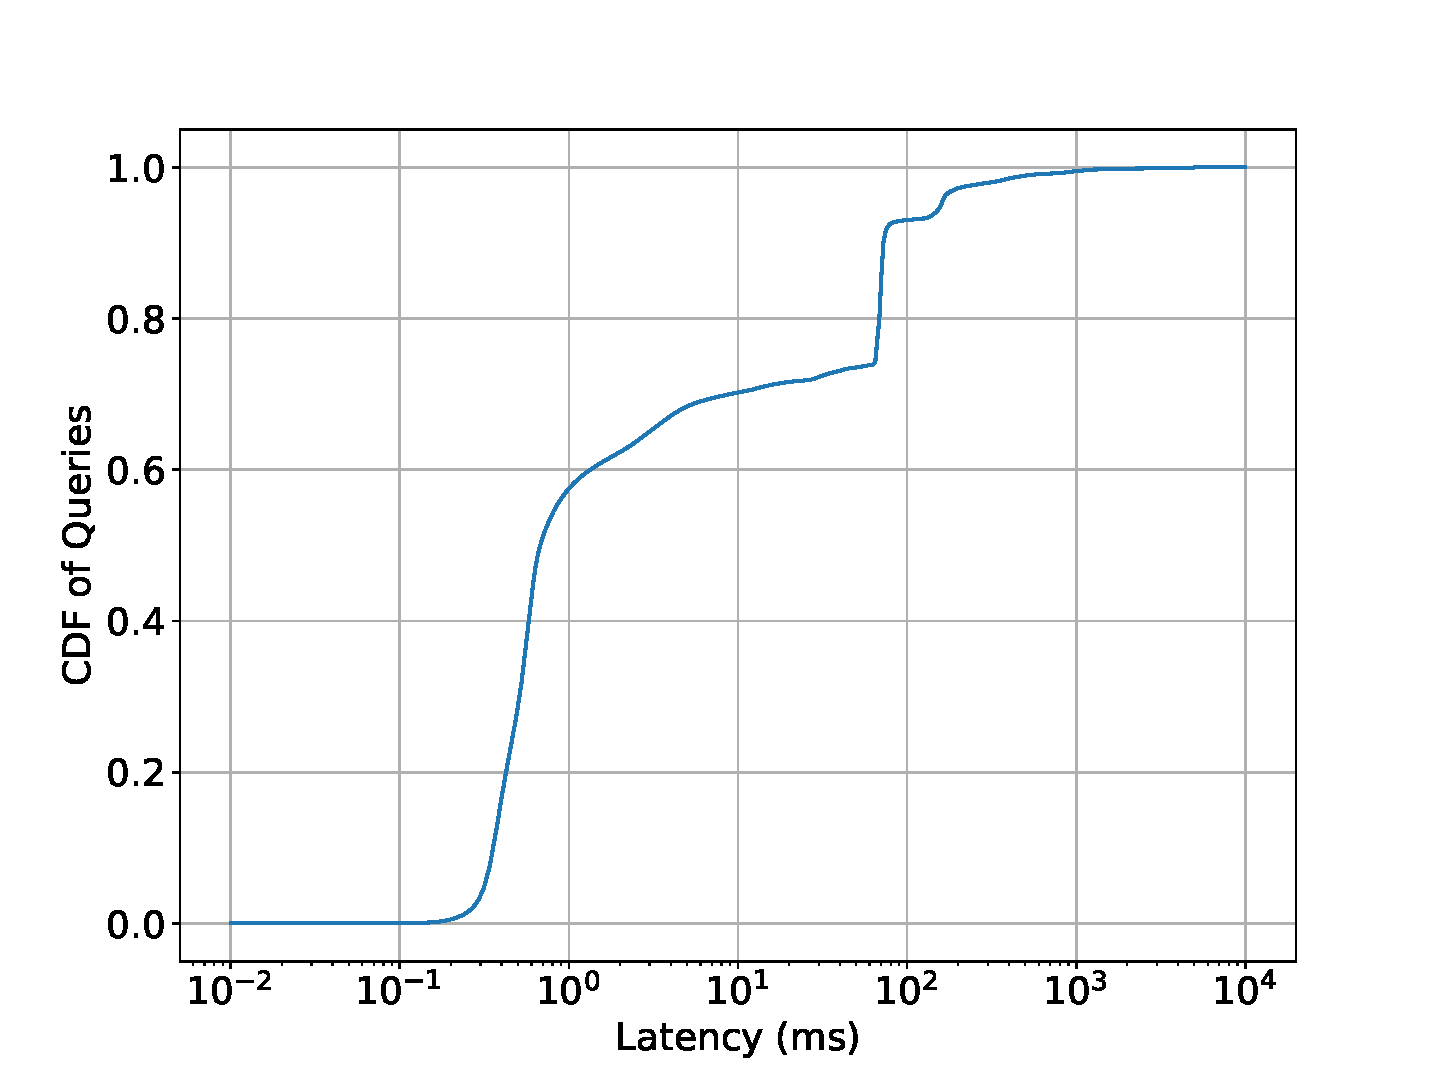
\includegraphics[width=0.45\textwidth]{figures/all_dns_latencies_isi.pdf}
    \caption{CDF of user DNS query latencies seen at a recursive resolve at ISI, over the course of one year. }
    \label{fig:all_dns_latencies_isi}
\end{figure}

\subsection{How Often Does a User Interact with the
Roots?}\label{how-often-does-a-user-interact-with-the-roots}

\label{sec:rr_close_look_discussion} From packet traces of all of 2018,
we would like to quantify the effect caching root DNS records has on
users, and how this differs from the ideal behavior users can
experience. Specifically, we are interested in the number of queries to
the root server as a fraction of user requests to the recursive
resolver. We refer to this metric as the cache miss rate, as it
approximates how often a TLD record is not found in the cache of the RR
in the event of a user query. We say approximately since, for example,
the recursive resolver may have sent multiple root requests per user
query, or root requests without any user query triggering them.

\begin{table}[]
\centering
\resizebox{.45\textwidth}{!}{%
\begin{tabular}{lll}
                                                             &                                                                                                                           &                             \\ \hline
\multicolumn{1}{|c|}{\multirow{3}{*}{\textbf{Assumptions}}}  & \multicolumn{1}{l|}{Web Page Load Time (ms)}                                                                              & \multicolumn{1}{l|}{3,000}  \\ \cline{2-3} 
\multicolumn{1}{|c|}{}                                       & \multicolumn{1}{l|}{Root DNS Latency (ms)}                                                                                & \multicolumn{1}{l|}{500}    \\ \cline{2-3} 
\multicolumn{1}{|c|}{}                                       & \multicolumn{1}{l|}{\begin{tabular}[c]{@{}l@{}}Number of DNS Look-Ups \\ Per Web Page\end{tabular}}                       & \multicolumn{1}{l|}{3}     \\ \hline
\multicolumn{1}{|l|}{\multirow{2}{*}{\textbf{Statistics}}}   & \multicolumn{1}{l|}{Number of User Queries (millions)}                                                                  & \multicolumn{1}{l|}{14.9}   \\ \cline{2-3} 
\multicolumn{1}{|l|}{}                                       & \multicolumn{1}{l|}{Number of Root Transactions}                                                                          & \multicolumn{1}{l|}{73,200} \\ \hline
\multicolumn{1}{|l|}{\multirow{3}{*}{\textbf{Implications}}} & \multicolumn{1}{l|}{\begin{tabular}[c]{@{}l@{}}Percent of user Queries \\ Resulting in a Root Transaction\end{tabular}} & \multicolumn{1}{l|}{.49}    \\ \cline{2-3} 
\multicolumn{1}{|l|}{}                                       & \multicolumn{1}{l|}{\begin{tabular}[c]{@{}l@{}}Expected Speed-up in PLT with \\ No Root Latency (ms)\end{tabular}}        & \multicolumn{1}{l|}{8}   \\ \cline{2-3} 
\multicolumn{1}{|l|}{}                                       & \multicolumn{1}{l|}{Resulting PLT Speedup (percent)}                                                                      & \multicolumn{1}{l|}{.25}   \\ \hline
\end{tabular}%
}
\caption{Statistics gathered from the ISI RR for a representative month of 2018, and implications of these statistics assuming conservative values for web page load time (PLT), root DNS latency, and number of DNS lookups per page. }


\label{tab:isi_cache_hit_rate_stats}
\end{table}

Relevant statistics and their implications on user-perceived latency are
presented in Table \ref{tab:isi_cache_hit_rate_stats}. We find that
daily cache miss rates of the resolver range from .1\% to 4.5\%, with a
median value of .5\%. This is quite a wide range of cache miss rates,
and is potentially skewed by the traffic generated by the internet
measurement lab (ISI). However, assessing the latency implications for
cache miss rates higher than the median is simply a multiplicative
factor and the qualitative conclusions are the same. \break \break
To calculate the impact of root latency on user experience, assume that
a web page load takes N seconds, that there are M serial DNS requests
per page, that the root latency is k seconds, and that the cache miss
rate is p.~Then, the resulting (average) latency due to root DNS
resolution per page load is given by \(pMk\), which, as a fraction of
PLT is \(\frac{p M k}{N}\). \break \break
Although N and k depend on a number of factors difficult to measure, p
can be measured for each recursive resolver (as shown in Table
\ref{tab:isi_cache_hit_rate_stats}), and M is relatively constant. To
demonstrate this last point, we performed page loads for 500 popular
domains using the Selenium web-browser and calculated the number of
blocking DNS requests per page load using methods in
\cite{sundaresan2013web}. We find 95\% of requests resulted in M
\(\leq\) 3 and so use this in what follows. \break
As exaggerated upper bounds on the impact of root DNS latency, we choose
N = 3 and k = .5
\footnote{ According to [http archive], RIPE Atlas, and the results from ISI itself, these are quite conservative estimates. }.
Hence, supposing root latency is completely removed from the equation, a
user saves, on average, 8 ms per page load. As a percentage of the total
page load time, this is .25\%, which is measurable, but not significant.
Note that for a conservative estimate of the cache miss rate of 4.5\%,
this would translate to approximately 2.3\% of a single page load.
\break \break
As a visualization of these results, Figure
\ref{fig:isi_root_dns_latency} shows a CDF of root DNS latency
experienced for queries over 2018. Requests that do not generate a query
to a root server are counted as having a root latency of 0.

\begin{figure}
    \centering
    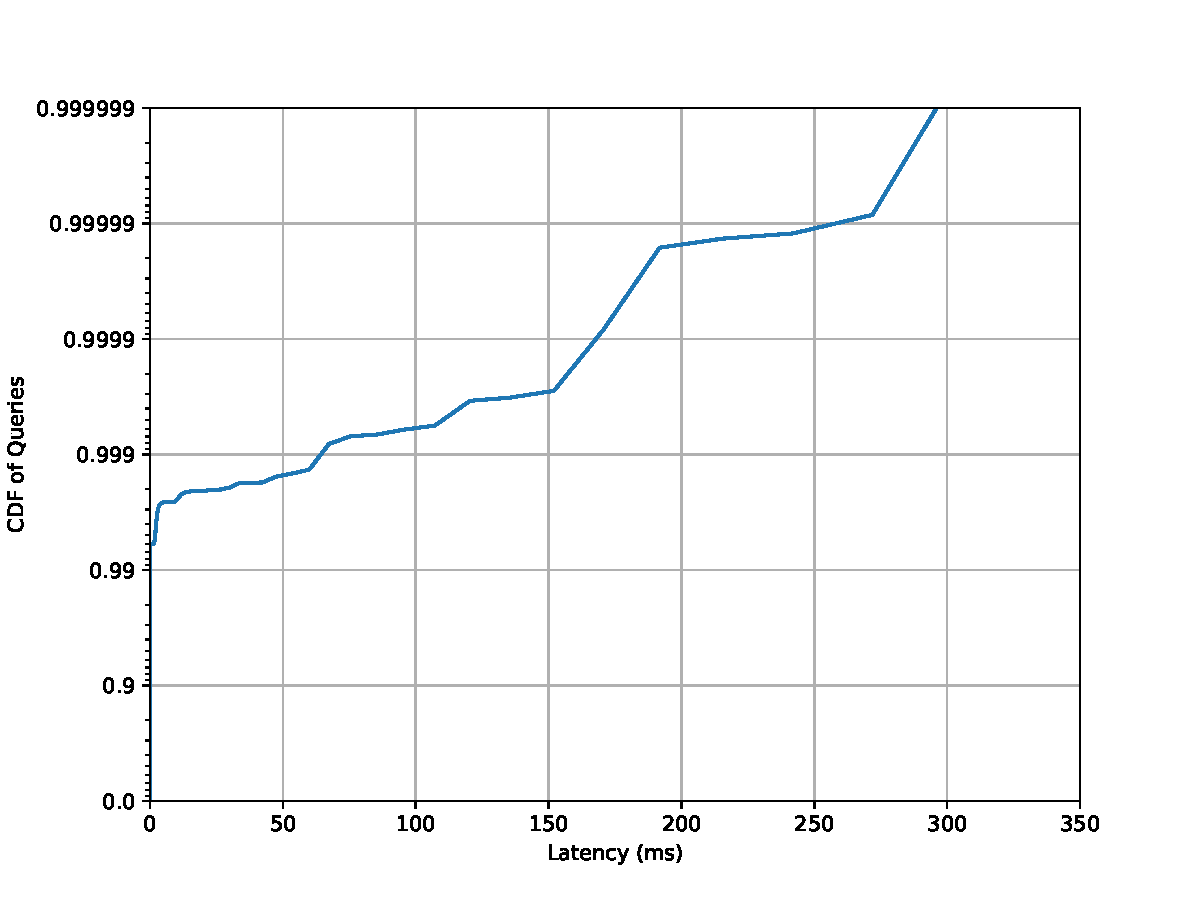
\includegraphics[width=0.45\textwidth]{figures/isi_root_dns_latency.pdf}
    \caption{Root DNS latency for queries made by users of the ISI recursive resolver during 2018. user queries that did not generate a query to a root server were given a latency of 0. }
    \label{fig:isi_root_dns_latency}
\end{figure}

Clearly the impact of root DNS latency in this situation is minimal, and
we can reasonably conclude that members of the ISI community do not
experience much latency due to the root DNS servers. Specifically,
Figure \ref{fig:isi_root_dns_latency} suggests it is particularly rare
for a user query to generate a query to a root DNS server. Further,
Table \ref{tab:isi_cache_hit_rate_stats} demonstrates that the latency
implications are small for the holistic user population. However, the
impact on user performance is not as small as one would expect. For
example, a particular day during January 2018 sees as many as 900
queries to the root server for the COM NS record. Given the 2 day TTL of
this record, this query frequency is absurdly large. This suggests that
heuristic arguments that users rarely experience root latency because
cached TLD records have long TTL's are not sufficient. \break 

\subsection{Case Study - Pointless Root Queries in BIND
9}\label{case-study---pointless-root-queries-in-bind-9}

\label{sec:pointless_queries_case_study} \textbf{TODO: Revise} Manual
inspection of specific query chains in the packet traces suggests that
certain logical flows in BIND can result in the root server being
unnecessarily queried. We are not making claims that BIND has
pathological bugs, since we did not explore the issue further. However,
this is an interesting area for future work.

\section{A Global Look at Root DNS
Latency}\label{a-global-look-at-root-dns-latency}

\label{sec:rr_global_look} Looking at cache hit rates of individual RR's
is informative, yet does not provide us with a notion of how much
latency large user populations experience in a day due to root DNS
resolution -- a statistic that would help us contextualize the effect of
anycast path inflation on user experience. Indeed it would be ideal if
we could measure the number of active users, how many times those users
request web pages and the cache hit rates of the users' recursive
resolvers to obtain an estimate of the latency they experience due to
root DNS resolution.

\subsection{Data Sources and
Processing}\label{data-sources-and-processing-1}

\label{sec:rr_global_look_data} Motivated by this ideal scenario, we
obtain statistics from a large CDN operator containing information about
the users of that CDN. Specifically, these statistics include RR IP's,
the number of distinct user IP's behind those RR's and the relative
query volume those user IP's contributed (as a fraction of the total CDN
query volume) for a month in 2019. Working with the notion of a ``user''
is valuable, as this provides us with an estimate of how much latency
each user experiences. Query volume is also of interest, since it is
correlated with activity on the web (and therefore likelihood of waiting
for a root DNS query). We saw no significant difference in the following
analysis when weighting by user counts or query volume, and so we weight
by user counts. We do note, however, that since the notion of user we
use is an IP address, one user can actually refer to several people
behind a NAT. \break \break
To leverage this CDN data in our aforementioned goal, we augment it with
traces from the 2018 Day in the Life of the Internet (DITL), organized
by OARC. DITL (run annually) contains concurrent packet captures from
all root servers except for G-root
\footnote{ A small portion of data from the 2018 DITL is missing or anonymized. We do not compensate for this, as the impact on the results is likely small. }
for two days in Spring. From DITL, we extracted the frequency of
requests each RR made to each root, the type of record requested, and
the domain requested. \break
Out of a total of 512 billion daily requests to all roots, we observed
310 billion daily requests for bogus domain names and 20 billion daily
requests for PTR records. Since these requests are not related to user
latency in most cases, we exclude them from the analysis.

\begin{table}[]
\centering
\resizebox{.45\textwidth}{!}{%
\begin{tabular}{|l|l|l|}
\hline
\textbf{Data Set}                            & \textbf{Statistic} & \textbf{Percent Representation} \\ \hline
\multirow{4}{*}{DITL $\cap$ CDN}             & DITL RR's          & 29.3                             \\ \cline{2-3} 
                                             & DITL Volume        & 71.9                            \\ \cline{2-3} 
                                             & CDN RR's           & 78.8                            \\ \cline{2-3} 
                                             & CDN Volume         & 88.1                            \\ \hline
\multirow{4}{*}{DITL $\cap$ CDN $\cap$ RIPE} & DITL RR's          & .14                              \\ \cline{2-3} 
                                             & DITL Volume        & 20.7                           \\ \cline{2-3} 
                                             & CDN RR's           & .34                              \\ \cline{2-3} 
                                             & CDN Volume         & 54.6                            \\ \hline
\end{tabular}%
}
\caption{Statistics displaying the extent to which the RR's of users in a large CDN represent RR's seen in the 2018 DITL captures. Also shown is the extent to which RR's of RIPE probes represent the 2018 DITL captures.}
\label{tab:dataset_matching_statistics}
\end{table}

We then join these data sets by /24, aggregating their respective user
IP counts and query volumes
\footnote{We take care to ensure that neither user counts nor query volumes are "double counted" across different IP's.}
-- this joined data set is referred to henceforth as the DCDN data set.
In the interest of data sanitation, we remove queries from prefixes in
the private IP space
\footnote{ The list we use can be found at \cite{private_ip_space}.}, as
these are not valid queries. Queries from these addresses account for
approximately 7\% of traffic to the roots. We additionally disregard the
presence of IPv6 traffic, and note that it comprises about 12\% of DITL
query volume. Finally, as previously mentioned, we do not consider
requests for bogus domain names nor requests for PTR records. Naturally,
there is a mismatch in the /24's represented by each data set. Table
\ref{tab:dataset_matching_statistics} summarizes the extent to which the
DCDN data (which is a subset of all users in the world) represents the
DITL captures, and vice versa. For brevity, we henceforth refer to these
/24's as RR's, even though each data point may represent several RR's.

\begin{figure}
    \centering
    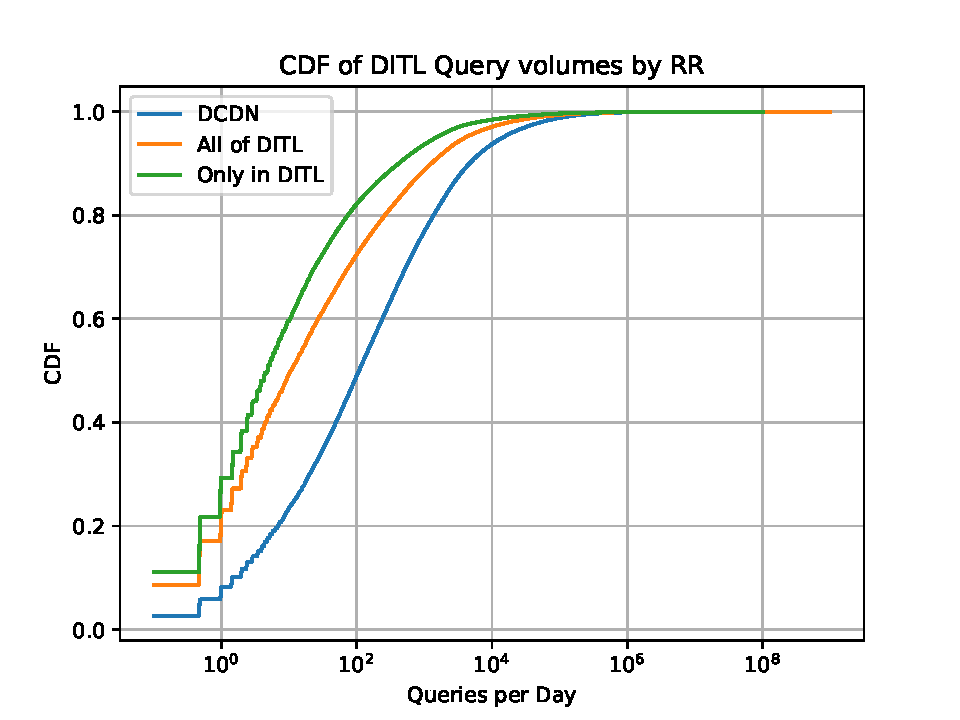
\includegraphics[width=0.45\textwidth]{figures/ditl_volume_comparisons.pdf}
    \caption{A comparison of daily query volumes seen from various sets of RR's. Those RR's both in the data set of the large CDN and DITL have relatively high daily query volumes, as evidenced by the large tail of DCDN. }
    \label{fig:ditl_volume_comparisons}
\end{figure}

Although the DCDN data considers a relatively small percentage of all
RR's, it captures a disproportionately large amount of all DITL volume.
A useful visualization of the effect of removing these RR's from
consideration is shown in Figure \ref{fig:ditl_volume_comparisons}.
Figure \ref{fig:ditl_volume_comparisons} is a CDF of daily query volumes
of RR's in the various data sets. The quartiles of the DCDN volume
counts (blue) are approximately 10-times those of DITL (orange),
suggesting /24s in the DCDN are a particularly high-querying subset of
all RR's. Therefore, as we will demonstrate in the following, despite
disregarding many RR's, our analysis actually provides an upper bound on
root DNS latency experienced by the typical user.

\subsection{Root Latency Experienced by
Users}\label{root-latency-experienced-by-users-1}

\label{sec:rr_global_look_analysis} Our main result, shown in Figure
\ref{fig:user_root_latency_per_day}, is a CDF of expected user latency
per day, where the expected value is calculated according to certain
assumptions we make about root latency.

{[}g{]}

\begin{figure}
    \centering
    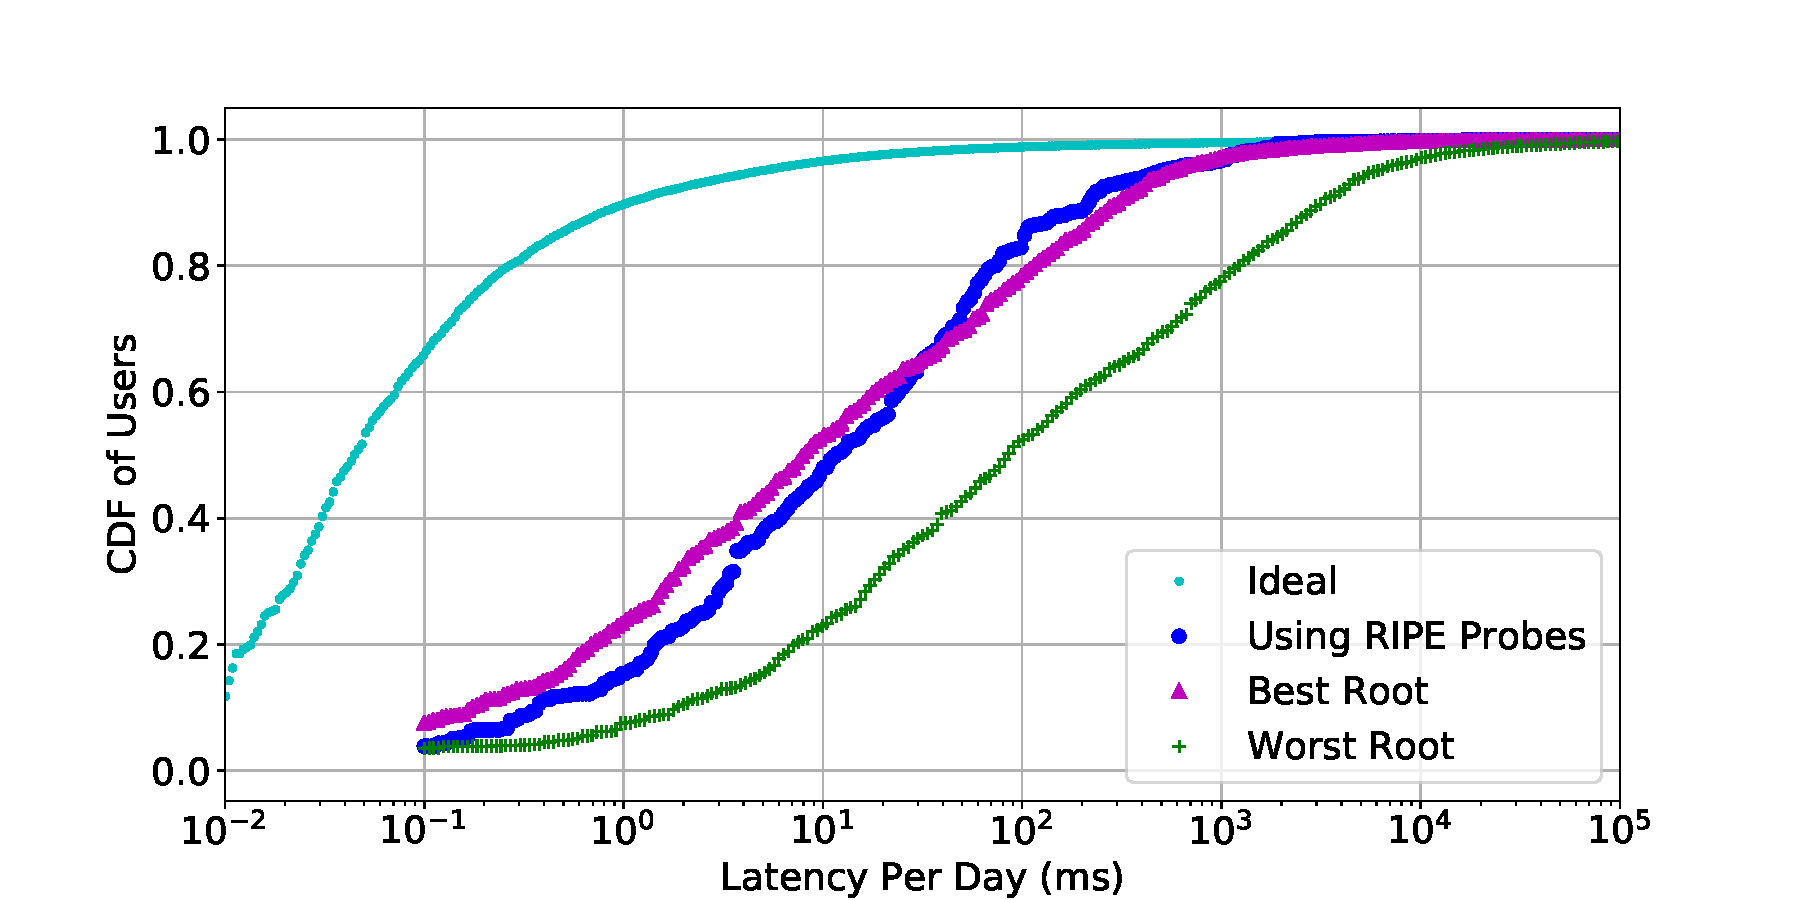
\includegraphics[width=0.45\textwidth]{figures/user_root_latency_per_day.pdf}
    \caption{A CDF of approximate latency a user experiences due to root DNS resolution, per day.}
    \label{fig:user_root_latency_per_day}
\end{figure}

To generate each line in Figure \ref{fig:user_root_latency_per_day}, the
expected root latency per RR per query is multiplied by the number of
queries per day each RR makes and divided by the number of users that RR
represents. The number of queries per day each RR makes is calculated
from DITL by first calculating daily query rates at each replica
(i.e.~total queries divided by total capture time) and subsequently
summing these rates across replicas. This product (representing daily
query latency per user) is then weighted by user count (from the CDN
data set) and the resulting CDF is calculated. Note the only detail
still unexplained is the way in which to estimate the expected root
latency per RR. \break \break
Since we do not know the actual latencies recursives saw to each replica
of each root, we use a few methods of estimating this expected latency,
each of which has its merits. As a useful comparison, we include lines
labeled ``basic-\textbf{N}'' which are generated naively assuming the
latency from every RR to every root server is \textbf{N} ms. For
example, the median latency incurred by a single user each day due to
root DNS resolution is 44 ms assuming a query from any RR to each root
is 80 ms. \break \break
The line labeled ``heuristic root value'' is calculated as follows:
assume each RR queries the set of roots according to a distribution
\(p_{RR}\), where \(p_{RR}\) is a discrete p.d.f. over the 12 root
servers indicating the probability with which the RR chooses each root
server to query. This p.d.f. is calculated empirically from the DITL
data. Next, obtain median latency values to each root (e.g.~from RIPE
Atlas) and call these \(l_{RR}\). Note that, for now, \(l_{RR}\) is
independent of RR. Compute the expected latency from each RR to any root
as the dot product between \(l_{RR}\) and \(p_{RR}\) (i.e.~the
expectation of the latency). Although somewhat imprecise, this method of
calculating latency for each user takes into account that some root
servers generally exhibit lower latencies than others due to investments
in infrastructure
\footnote{ For example, at the time of writing the median latency to B root (3 sites) is 130ms whereas the median latency to F root  (225 sites) is less than 5 ms. }.
Hence, this line can be considered a more reasonable estimate of the
latency users experience due to root DNS resolution. This is
corroborated by the ``middle-of-the-pack'' median estimate of 15 ms/day.
\break \break
The line labeled ``RIPE'' looks only at those RR's in both the DITL and
CDN data sets housing RIPE probes. We are interested in RIPE probes,
since RIPE probes routinely issue ping measurements to each root server
and report latency values. Note that we were able to determine the RR
for a subset of all active RIPE probes. Further, the set of RR's housing
a RIPE probe did not overlap perfectly with RR's in the DCDN data set.
Using our notation from the previous paragraphs, \(l_{RR}\) is then
populated from these ping measurements for each RR, and the expected
root latency per query is calculated per RR according to \(p_{RR}\).
From Table \ref{tab:dataset_matching_statistics}, we see that /24's
housing RR's of RIPE probes only account for 21\% of the volume in DITL,
and about .1\% of all /24's; hence, RIPE probes are not representative
of the population (as expected). However, for users in these /24's, this
is a fairly accurate measurement of the expected daily latency due to
root DNS resolution. Additionally, many studies, e.g.
\cite{li_levin_spring_bhattacharjee_2018}, use RIPE probes when
measuring anycast latency/inefficiency so this line could provide a
useful comparison. We see this method provides one of the lowest median
estimates of 12 ms/day. This makes sense, as RIPE probes generally
reside in well connected areas of Europe. \break \break
Finally, the line labeled `ideal' does not use DITL query volumes to
calculate daily user latency, but instead represents some hypothetical
scenario in which each RR queries for all TLD records exactly once per
TTL. The resulting hypothetical median daily latency of .23 m{[}h{]}s
could represent a future in which caching works at recursives as
intended.

\section{Anycast Path Inflation}\label{anycast-path-inflation}

\label{sec:api} Anycast path inflation is a concept introduced in
\cite{de2017anycast} and expanded upon in
\cite{li_levin_spring_bhattacharjee_2018}, which measures how
inefficiently queries to anycasted IP's are mapped to physical replicas.
We use the definition from \cite{li_levin_spring_bhattacharjee_2018},
which breaks down path inflation into unicast path inflation (UPI) and
anycast path inflation (API). UPI measures the extra latency a query
incurs as a result of not being mapped to the geographically closest
physical replica. API measures the additional latency incurred beyond
the optimal unicast alternative. API for a query to an anycasted address
can be large, which (generally) occurs when queries are routed to
geographically distant replicas, despite the existence of a close
replica. \break
We have demonstrated that, due to caching, users do not experience much
root latency. Since prior work has focused on inflation (and how it
affects users), we further wish to estimate API incurred by users of
recursives around the world due to the root DNS servers. Furthermore, we
wish to compare this API to inflation incurred by users of a large
anycast CDN, to provide perspective as to how this inflation impacts
users.

\subsection{Root DNS API}\label{root-dns-api}

\label{sec:api_root} To measure anycast inflation for the root DNS
deployment, we again leverage the DITL captures. The DITL captures are a
rich source of data for this purpose because they provide us with a
global view of which recursives are accessing which locations for all
but a small subset of root DNS sites
\footnote{Notably excluded from this analysis is H root, which did not provide packet traces at the per-site level.}.

\iffalse

Talk about daily inflation due to root DNS * Custom geolocating of
public DNS IPs Talk about inflation per query of root DNS vs anycast DNS
Talk about accuracy/validation of methods

\fi

\section{Discussion}\label{discussion}

\subsection{Approximations and
Limitations}\label{approximations-and-limitations}

\label{sec:discussion_approximations} In the above we have attempted to
provide upper bounds of the impact of user latency on user experience.
The reason for this is two-fold. First, what we are trying to measure
can only be measured by accumulating measurements from a variety of
sources and so naturally we have a lack of representativeness and
certainty when discussing results. Second, we are arguing that users
rarely interact with the DNS infrastructure. Hence, we would like to
obtain upper bounds on latency experienced by users due to root DNS
resolution, so we can make claims with more certainty. \break \break
The notable limitations in our above analysis are

\begin{enumerate}
        \item In the case of studying root record cache hit rates at the resolver level, we were only able to study one recursive resolver.
        \item When looking at global root server querying behavior, we were only able to calculate daily user latency due to root DNS resolution for approximately 30% of (v4) recursive resolvers around the world. 
\end{enumerate}

However, even when we use extremely conservative estimates of parameters
such as page load time, or root DNS latency we find in Section
\ref{sec:rr_close_look_discussion} that root DNS resolution adds a
\textit{negligible} latency to page loads. \break
One might also consider a lack of insight into what latencies each
recursive resolver saw to be a weakness of our analysis. However,
regardless of which method is used to calculate expected daily user
latency, users generally experience median values of \(<\) 50 ms/day
while worst case users generally experience \(<\) 10 s/day. Moreover,
recall the following simplifications we make in our above (global)
analysis.

\begin{enumerate}
        \item Requests to root servers are generated by a myriad of services, so each request may not have been generated by an actual user.
        \item The notion of "user" here (in the CDN) is likely a home router, potentially representing several users across many devices.
        \item The DCDN data set contains particularly "active" RR's.
\end{enumerate}

To investigate item 2 in the above list, we looked specifically at
recursive resolvers in AS's owned by mobile providers in the United
States. Many large mobile providers in the U.S. do not assign IPv4
addresses to individual devices, and so act as giant NAT's.
Additionally, U.S. mobile providers have separate AS's for their mobile
networks. For this, we use the free IP to ASN mapping service provided
by MaxMind. We find that the daily user latency of these particular
recursives is indeed orders of magnitude over the median. Since we have
no reason to believe mobile Internet traffic generates more root
requests than any other type of traffic, this confirms our suspicions
that user count estimates for NAT'ed networks are lower bounds. \break
This further establishes that Figure \ref{fig:user_root_latency_per_day}
is to be interpreted as a conservative upper bound of daily root latency
experienced by users.

\subsection{Root DNS in Anycast}\label{root-dns-in-anycast}

\label{sec:discussion_implications} In the context of anycast, recall
that studies routinely use the root servers as sources of data. However,
in light of these results, one can question whether the typical user
interacts with these particular anycast deployments. One could go
further to argue the utility of proposed improvements to IP anycast
should not be assessed using root DNS servers, as the generalization
ability of the improvement to all IP anycast systems is uncertain.
\break
Regardless, we believe these results should encourage others to consider
the implications of anycasts' weakness, whatever they may be. Pointing
out sub-optimal performance for the sake of analysis is interesting, but
it is equally interesting to note whether or not this sub-optimal
performance has any practical, measurable effect.

\section{Related Work}\label{related-work-1}

\label{sec:related} IP anycast performance is usually studied in the
context of two applications: the root DNS servers, and CDN's. In
addition to these topics, we discuss studies of popular recursive
resolvers, and user-centric measurements of web performance.

\subsection{Root DNS Anycast
Performance}\label{root-dns-anycast-performance}

The performance of anycast in the context of root DNS is generally
gauged by anycast's ability to balance load among server replicas or
provide low latency to users. Generally, all studies conclude that
anycast successfully balances load, while latency performance depends on
the specific deployment configuration. \cite{moura2016anycast} looks at
a DDoS attack on the root name server infrastructure, and generally
shows that anycast is a good defense mechanism against such attacks. An
earlier study, \cite{sarat2006use} confirms that anycast protects the
root DNS infrastructure against such attacks and, furthermore, that
anycast routes users to an optimal location in most cases.
\cite{de2017anycast} looks at user latency to C, F, K, and L-root and
attributes better performance to good geographic location and peering
strategies. These findings coincide with an earlier study,
\cite{ballani2006measurement}, who conclude the performance of anycast
is intrinsically linked to deployment strategy. Additionally
\cite{de2017anycast} finds that as few as 12 sites can provide ``good''
latency to users. \cite{li_levin_spring_bhattacharjee_2018},
\cite{colitti2006evaluating}, \cite{de2017anycast}, and
\cite{liang2013measuring} are all examples of studies who quantify
latencies to various root servers, and note how these compare to the
(optimal) latency of the closest unicast alternative for the user who
issued the query.

\subsection{CDN Anycast Performance}\label{cdn-anycast-performance}

Some CDN's (e.g.~Cloudflare, Edgecast, Fastly) use IP anycast to augment
their serving infrastructure. When deploying an Anycast CDN (ACDN),
delivering content to users with low latency becomes a high priority, as
there is a large financial incentive to do so. The simplicity of IP
anycast comes at the cost of having coarse grained control over where
user queries land. Shifting user load between nodes during peak hours,
for example, is a challenging problem. As a potential solution,
\cite{alzoubi2011practical} and \cite{flavel2015fastroute} use DNS
redirects at ADNS servers to shift load among anycast nodes, albeit in
slightly different ways. \cite{calder2015analyzing} analyzes what
latency users are achieving, compared to optimal, when being routed to
anycast nodes and finds that 10\% of users experience a latency
inflation of at least 100 ms.

\subsection{Recursive Resolvers and the Benefits of
Caching}\label{recursive-resolvers-and-the-benefits-of-caching}

Similar to the RR analysis conducted here, \cite{jung2002dns} looks at
DNS traffic on a small network and notably finds that 16\% of queries
resulted in queries to the root, most of which were for invalid domains.
As this study is quite old, it is no surprise that this rate has
decreased (recall we observed .5\% of queries resulted in queries to the
root) since browser designers and network engineers understand the
importance of caching. \cite{callahan2013modern} also looks at a RR and
analyzes statistics of DNS exchanges occurring over it including DNS
transaction latencies. Both \cite{yu2012authority} and \cite{lentz2013d}
look at certain pathological behaviors of popular recursive resolvers,
and the implications these behaviors have on root DNS load.

\subsection{Web Performance}\label{web-performance}

Although we were unable to find any specific study that looked at how
web performance and root DNS latency were related, there are certainly
studies characterizing web performance. \cite{sundaresan2013web}
characterizes web performance bottlenecks in (at the time) new broadband
networks, and finds that latency is the main bottleneck for PLT when the
user's bandwidth exceeds 16 Mbps. However, the study does not
realistically emulate a page load and, in particular, can not analyze
the effect of having multiple DNS resolutions per page. Similarly,
\cite{asrese2016wepr} analyzes how each step of a page load contributes
to the aggregate PLT using a tool designed in-house. However, unlike
\cite{sundaresan2013web}, they did not conduct a large measurement
campaign and do not include information about multiple DNS lookups per
page. A more recent study, \cite{enghardt2019web} provides a brief
survey of web performance measurement studies and explains why it is
difficult (with current practices) to compare two different studies in
web performance.

\iffalse

(studies looking at anycast in context of root DNS servers) Anycast
Performance, Problems and Potential how many sites are enough? A
measurement based deployment proposal for IP Anycast Evaluating the
Effects of Anycast on DNS Root Nameservers Measuring Query Latency of
Top Level DNS Servers Anycast vs.~DDoS: Evaluating the November 2015
Root DNS Event On the Use of Anycast in DNS (studies looking at anycast
in context of CDN's) fastroute A Practical Architecture for an Anycast
CDN Edgecast paper that hasn't been released yet Analyzing the
Performance of an Anycast CDN (studies looking at recursive
resolvers/caching) (maybe) John's TR of how different resolvers query at
different times On Modern DNS Behavior and Properties DNS Performance
and the Effectiveness of Caching D-mystifying the D-root Address Change
Authority Server Selection of DNS Caching Resolvers{[}i{]} Recursives in
the Wild: Engineering Authoritative DNS Servers (studies looking at web
performance/how user caching effects it) Measuring and mitigating web
performance bottlenecks in broadband access networks WePR: A tool for
Automated Web Performance Measurement Demystifying Page Load Performance
with WProf{[}j{]} Practical Challenge Response for DNS DNS Resolvers
Considered Harmful{[}k{]} Studies looking at root servers and queries
that land at them On eliminating root nameservers from the DNS DNS
Measurements at a Root Server A Day at the Root of the Internet

\fi

\section{Conclusion}\label{conclusion-1}

IP anycast has come under attack, with studies showing, for example, how
BGP can naturally route users to suboptimal anycast instances and
inflate user latencies. Due to the relative availability of root DNS
data and diverse deployment strategies of the root DNS servers, they are
common targets for delineating inefficiencies and suggesting
improvements to IP anycast. We argue not only that the root DNS servers
have different design goals (i.e.~resiliency against attacks) than that
of other anycast services, but also that users rarely interact with the
root DNS infrastructure -- rendering perceived inefficiencies and
proposed improvements to be ill-founded when only tested on the root
DNS. Perhaps simple yet effective ideas such as browser link prefetching
or DNS request parallelization should be expanded and their adoption by
users encouraged, rather than proposed improvements to IP anycast.
{[}a{]}ideally we would control the linebreak in the latex so it occurs
after ``it,'' {[}b{]}this argument about prior studies needs to be more
careful, I think. I propose an alternate abstract below {[}c{]}perhaps
add others {[}d{]}does markdown not handle blank-lines as paragraph
breaks? this \break\break stuff is a step backwards. {[}e{]}we have to
be careful about this statement. ``has its drawbacks'' is really
vague--every study has drawbacks. I think the point is stronger: the
IMPLICATION of these studies is performance is much worse than it could
be and people are suffering. We show that (1) no, it doesn't matter for
the root.

But we need to go further than that. Does the root STAND IN for other
anycast systems? Even if the root isn't slow in practice, would
cloudflare be slow? (2) we need to say how we think our results should
generalize (or that they only apply to the root) {[}f{]}again,
``contextualize resarch'' : who cares. Our goal is (I think) to show
that concerns raised about the root latency are greatly exaggerated.
ALSO we need to pick out a specific claim or two, and say what we think
to be a more represntive number. That is: we need to find a number like
100ms and show that 2ms is what is perceived. {[}g{]}update labels in
legend {[}h{]}assumed 80 ms per query -- should comment on this, or just
quote the expected number of queries per day, this might be more
intuitive {[}i{]}interesting that in 10 minutes they observe so many
queries for COM TLD yet don't see any issue with that {[}j{]}Might be an
interesting tool to use {[}k{]}Mark shared in an email -- shows time
between DNS queries \& TCP connection starts can be big, which suggests
DNS is not blocking

\bibliography{bib.bib}

\end{document}
